\documentclass[wide,a4paper,titlepage,12pt]{mwart}
\usepackage{polski,graphicx,pdflscape}
\usepackage[utf8]{inputenc}
\usepackage{multirow}

\title{Wyznaczanie współczynnika lepkości cieczy na podstawie prawa Stokesa}
\author{Tymon Tobolski (181037)\\Jacek Wieczorek (181043)}

% Title page layout (fold)
\makeatletter
\renewcommand{\maketitle}{
\begin{titlepage}
  \begin{center}
    \vspace*{3cm}
    \LARGE Laboratorium Podstaw Fizyki \par
    \vspace{1cm}
    \normalsize Numer ćwiczenia: 8 \par
  \end{center}

  {\bf Temat ćwiczenia:} Wyznaczanie współczynnika lepkości cieczy na podstawie prawa Stokesa \par
  {\bf Nazwisko i imię prowadzącego kurs:} mgr Paulina Kamyczek \par

  %   \normalsize \@author\par \normalsize
  %   \vspace{3cm}
    \vspace{2cm}
  %   Wydział Elektroniki\\ II rok\\ śr 9:15--11:00 \par
  %   \vspace{5cm}
  %   \small \@date


  \begin{table}[h]
    \begin{center}
      \begin{tabular}{|c|c|}
			\hline
			Wykonawca:	& \\
			\hline
			Imię i nazwisko, & Tymon Tobolski 181037 \\
			nr indeksu, wydział & Jacek Wieczorek 181043 \\
			& Wydział Elektroniki \\
			\hline
			Termin zajęć: dzień tygodnia, godzina &	3.11.2010 środa 9.15-11.00 \\
			\hline
			Numer grupy ćwiczeniowej &	5 \\
			\hline
			Data oddania sprawozdania:	& \\
			\hline
			{\bf Ocena końcowa} & \\
			\hline
      \end{tabular}
    \end{center}
  \end{table}
 \vspace{2cm}
	Zatwierdzam wyniki pomiarów. \par
	Data i podpis prowadzącego zajęcia: ................................................................................... \par

 \vspace{2cm}
{\bf Adnotacje dotyczące wymaganych poprawek oraz daty otrzymania poprawionego sprawozdania}

\end{titlepage}
}
\makeatother
% Title page layout (end)

\begin{document}
  \maketitle

  \section{Cel ćwiczenia} % (fold)
  \label{sec:Cel}
    Celem ćwiczenia jest wyznaczenie współczynnika lepkości przykładowej cieczy za pomocą pomiaru czasu spadania kulki w cylindrycznym naczyniu wypełnionym cieczą oraz za pomocą wiskozymetru Hopplera. 
    
    
  % section Wstęp (end)
  
  \section{Pomiar współczynnika lepkości cieczy za pomocą szklanego naczynia cylindrycznego}
  
    \subsection{Pomiar średnicy i masy kulek oraz obliczenie gęstości}
    
    Pomiar średnicy $d$ kulek został wykonany za pomocą suwmiarki, dziesięciokrotnie dla każdej z trzech kulek. Masa $m$ została określona przy wykorzystaniu wagi elektronicznej. Wyniki pomiarów znajdują się w tabeli \ref{rozmiary}.
    \newline
  
    \begin{table}[hp]
      \begin{center}
        \begin{tabular}{|c|c|c|c|c|c|c|c|c|c|}
          \hline
            $Kulka$	 &
            $m[g]$	 &
            $\Delta m[g]$	 &
            $d[mm]$	 &
            $\bar{d}[mm]$	 &
            $\Delta \bar{d}[mm]$	 &
            $\bar{r}[mm]$	 &
            $\Delta \bar{r}[mm]$	 &
            $\rho_k[g/cm^3]$ &
            $\Delta \rho_k[g/cm^3]$ \\
          \hline
            \multirow{10}{*}{1} &
            \multirow{10}{*}{0,283} &
            \multirow{10}{*}{0,0002} &
            5,6 &
            \multirow{10}{*}{5,72} &
            \multirow{10}{*}{0,0063} &
            \multirow{10}{*}{2,86} &
            \multirow{10}{*}{0,0032} &
            \multirow{10}{*}{2,888} &
            \multirow{10}{*}{0,012} \\
            & & & 5,7 & & & & & &\\
            & & & 5,7 & & & & & &\\
            & & & 5,8 & & & & & &\\
            & & & 5,8 & & & & & &\\
            & & & 5,8 & & & & & &\\
            & & & 5,7 & & & & & &\\
            & & & 5,6 & & & & & &\\
            & & & 5,7 & & & & & &\\
            & & & 5,8 & & & & & &\\
          \hline
            \multirow{10}{*}{2} &
            \multirow{10}{*}{0,233} &  
            \multirow{10}{*}{0,0002} &
            5,8 &
            \multirow{10}{*}{5,86} &
            \multirow{10}{*}{0,01} &
            \multirow{10}{*}{2,93} &
            \multirow{10}{*}{0,005} &
            \multirow{10}{*}{2,211} &
            \multirow{10}{*}{0,013} \\
            & & & 5,8 & & & & & &\\
            & & & 5,9 & & & & & &\\
            & & & 6,0 & & & & & &\\
            & & & 5,8 & & & & & &\\
            & & & 5,9 & & & & & &\\
            & & & 5,7 & & & & & &\\
            & & & 5,8 & & & & & &\\
            & & & 5,9 & & & & & &\\
            & & & 6,0 & & & & & &\\
          \hline
            \multirow{10}{*}{3} &  
            \multirow{10}{*}{0,7168} & 
            \multirow{10}{*}{0,0002} & 
            8,0 &  
            \multirow{10}{*}{8} &  
            \multirow{10}{*}{0,014} &  
            \multirow{10}{*}{4.0} &  
            \multirow{10}{*}{0,07} & 
            \multirow{10}{*}{2,674} &  
            \multirow{10}{*}{0,015} \\
            & & & 7,9 & & & & & &\\
            & & & 8,2 & & & & & &\\
            & & & 8,1 & & & & & &\\
            & & & 7,9 & & & & & &\\
            & & & 8,0 & & & & & &\\
            & & & 8,1 & & & & & &\\
            & & & 8,0 & & & & & &\\
            & & & 7,8 & & & & & &\\
            & & & 8,0 & & & & & &\\
          \hline
        \end{tabular}
        \caption{\label{rozmiary}Wyniki pomiarów masy oraz średnicy kulek}
      \end{center}
    \end{table}
    
    Wykorzystane wzory:
    
    \begin{eqnarray*}
      \bar{d} &=& \frac{1}{n} \sum_{i=1}^{n} d_i \\
      \Delta \bar{d} &=& \sqrt{\frac{1}{n(n-1)} \sum_{i=1}^{n} (d_i - \bar{d})^2} \\
      \bar{r} &=& \frac{\bar{d}}{2} \\
      \Delta \bar{r} &=& \frac{\Delta \bar{d}}{2} \\
      \rho_k &=& \frac{m}{\frac{4}{3} \pi r^3} \\
      \Delta \rho_k &=& \left [ \left | \frac{\Delta m}{m}\right | + \left | \frac{3\Delta r}{r}\right |\right] \rho_k
    \end{eqnarray*}
    
    Przykładowe obliczenia (kulka nr 1):
    
    \begin{eqnarray*}
      \bar{d} &=& \frac{5,6 + ... + 5,7}{10} = 5,72 mm \\
      \Delta \bar{d} &=& \sqrt{\frac{1}{10*(10-1)} \left[ \left( 5,6 - 5,72\right)^2 + ... + \left( 5,7 - 5,72\right)^2  \right] }  = 0,00622222 \approx 0,0063 mm \\
      \bar{r} &=& \frac{5,72}{2} = 2,86 mm \\
      \Delta \bar{r} &=& \frac{0,0063}{2} \approx 0,0032 mm \\
      \rho_k &=& \frac{0,283}{\frac{4}{3} \pi (0,286)^3} = 2,888 \frac{g}{cm^3} \\
      \Delta \rho_k &=& \left [ \left | \frac{0,0002}{2,888}\right | + \left | \frac{3*0,00032}{0,286}\right |\right] \rho_k = 0,011465 \approx 0,012 \frac{g}{cm^3}
    \end{eqnarray*}
    
    \subsection{Pomiar czasu spadania kulek w naczyniu}
    
  
    Pomiar został wykonany za pomocą stopera, dziesięciokrotnie dla każdej kulki osobno. Zmierzony został czas $t$, w którym każda z kulek pokonuje spadając w cieczy określony dystans $h$. Wyniki pomiarów znajdują się w tabeli \ref{czas}.
    \newline

    Wykorzystane wzory:
    
    \begin{eqnarray*}
      \bar{t} &=& \frac{1}{n} \sum_{i=1}^{n} t_i \\
      \Delta \bar{t} &=& \sqrt{\frac{1}{n(n-1)} \sum_{i=1}^{n} (t_i - \bar{t})^2} \\
    \end{eqnarray*}
    
    Przykładowe obliczenia (kulka 1):
    
    \begin{eqnarray*}
      \bar{t} &=& \frac{1}{n} \sum_{i=1}^{n} t_i = 8,298 s\\
      \Delta \bar{t} &=& \sqrt{\frac{1}{10*(10-1)} \sum_{i=1}^{10} (t_i - 8,298)^2} = 0,0245955 \approx 0,025 s \\
    \end{eqnarray*}
    
    Obliczenie współczynnika lepkości:
    
    \begin{eqnarray*}
      g &=& 9,81 \frac{m}{s^2} \\
      h &=& 24,8 cm = 0,248 m \\
      \rho_c &=& 1,25 \frac{g}{cm^3} \\
      \eta &=& \frac{2r^2 * g * t * (\rho_k - \rho_c)}{9h} \\
      \\
      \eta_1 &=& \frac{2*(2,86 * 0,001)^2 * 9,81 * 8,298 * (2,888 - 1,25)*10^3}{9*0,248} = 0,9773 \frac{kg}{s*m}\\
      \eta_2 &=& \frac{2*(2,93 * 0,001)^2 * 9,81 * 13,145 * (2,211 - 1,25)*10^3}{9*0,248} = 0,9537 \frac{kg}{s*m}\\
      \eta_3 &=& \frac{2*(4 * 0,001)^2 * 9,81 * 5,086 * (2,674 - 1,25)*10^3}{9*0,248} = 1,0185 \frac{kg}{s*m}\\
      \\
      \Delta \eta &=& \left |  \frac{4rgt(\rho_k-\rho_c)\Delta r}{9h}  \right | +      \left |  \frac{2r^2g(\rho_k-\rho_c)\Delta t}{9h}  \right | +      \left |  \frac{2r^2gt\Delta \rho_k}{9h}  \right | +      \left |  \frac{2r^2gt\Delta \rho_c}{9h}  \right | +      \left |  \frac{2r^2gt(\rho_k-\rho_c)\Delta h}{9h^2}  \right | \\
      \\
      \Delta \eta_1 &=& 0,0022 \frac{kg}{s*m}\\
      \Delta \eta_2 &=& 0,0031 \frac{kg}{s*m}\\
      \Delta \eta_3 &=& 0,0035 \frac{kg}{s*m} \\
      \\
      \bar{\eta} &=& 0,983 \frac{kg}{s*m} \\
      \Delta \bar{\eta} &=& 0,024 \frac{kg}{s*m} \\
    \end{eqnarray*}
    \clearpage
    
    \begin{table}
      \begin{center}
        \begin{tabular}{|c|c|c|c|}
          \hline
            $Kulka$ &
            $t[s]$ &
            $\bar{t}[s]$ &
            $\Delta \bar{t}[s]$ \\
          \hline
          	\multirow{10}{*}{1} &
            8,37 &
            \multirow{10}{*}{8,298} &
            \multirow{10}{*}{0,025} \\
            & 8,47 & & \\
            & 8,36 & & \\
            & 8,42 & & \\
            & 8,24 & & \\
            & 8,24 & & \\
            & 8,40 & & \\
            & 8,10 & & \\
            & 7,98 & & \\
            & 8,40 & & \\
          \hline
            \multirow{10}{*}{2} &
            13,20 &
            \multirow{10}{*}{13,145} &
            \multirow{10}{*}{0,036} \\
            & 13,09 & & \\
            & 13,51 & & \\
            & 13,11 & & \\
            & 13,28 & & \\
            & 13,27 & & \\
            & 13,13 & & \\
            & 12,87 & & \\
            & 12,89 & & \\
            & 13,10 & & \\
          \hline
            \multirow{10}{*}{3} &
            5,11 &
            \multirow{10}{*}{5,086} &
            \multirow{10}{*}{0,009} \\
            & 5,1 & & \\
            & 5,15 & & \\
            & 5,07 & & \\
            & 5,01 & & \\
            & 4,99 & & \\
            & 4,99 & & \\
            & 4,99 & & \\
            & 5,21 & & \\
            & 5,24 & & \\
          \hline
        \end{tabular}
      \end{center}
      \caption{\label{czas}Wyniki pomiarów czasu spadania kulek.}
    \end{table}
    
    \begin{table}
      \begin{center}
        \begin{tabular}{|c|c|c|c|c|}
          \hline
            $Kulka$ &
            $\eta[kg/(s*m)]$ &
            $\Delta \eta[kg/(s*m)]$ &
            $\bar{\eta}[kg/(s*m)]$ &
            $\Delta \bar{\eta}[kg/(s*m)]$ \\
          \hline
          	1 & 0,9773 & 0,0022 & \multirow{3}{*}{0,983} & \multirow{3}{*}{0,024} \\
          	2 & 0,9537 & 0,0031 & & \\
            3 & 1,0185 & 0,0035 & & \\
          \hline
        \end{tabular}
      \end{center}
      \caption{\label{lepkosc1} Obliczone wartości współczynnika lepkości.}
    \end{table}
    
  \clearpage 
  \section{Wyznaczanie współczynnika lepkości cieczy przy pomocy wiskozymetru}
    Pomiar został dokonany z wykorzystaniem stopera. Zmierzony został czas $t$, w którym kulka umieszczona w wiskozymetrze pokonała oznaczony dystans. Pomiar został powtórzony pięciokrotnie. Wyniki znajdują się w tabeli \ref{wisko}.
   
   
    \begin{table}[h]
      \begin{center}
        \begin{tabular}{|c|c|c|c|c|c|c|c|c|}
          \hline
            Lp & 
            $t [s]$ & 
            $\bar{t} [s]$ &
            $\Delta \bar{t}[s]$ &
            $k [m^2 / s^2]$ &
            $\rho_k [kg/m^3]$ & 
            $\Delta \rho_k [kg/m^3]$ &
            $\rho_c [kg/m^3]$ & 
            $\Delta \rho_c [kg/m^3]$  \\
          \hline
            1 &	162,78 & 
              \multirow{5}{*}{161,76} &
              \multirow{5}{*}{1,0} &
              \multirow{5}{*}{0,0000001216} &
              \multirow{5}{*}{8120} &
              \multirow{5}{*}{10} &
              \multirow{5}{*}{1235} &
              \multirow{5}{*}{5} \\
            2	& 162,62 & & & & & & & \\
            3	& 161,26 & & & & & & & \\
            4	& 160,5  & & & & & & & \\
            5 &	161,62 & & & & & & & \\
          \hline
        \end{tabular}
      
      \end{center}
          \caption{\label{wisko} Wyniki pomiarów czasu spadania kulki.}
    \end{table}
    
    Wykorzystane wzory i obliczenia:
    
    \begin{eqnarray*}
      \bar{t} &=& \frac{1}{n} \sum_{i=1}^{n} t_i = 161,76 s\\
      \Delta \bar{t} &=& \sqrt{\frac{1}{n(n-1)} \sum_{i=1}^{n} (t_i - \bar{t})^2} \approx 1,0 s\\ \\
      \eta &=& k*(\rho_k - \rho_c) * t = 0,1354 \frac{kg}{s*m}\\
      \Delta \eta &=& \left |k*t*\Delta \rho_k \right | + \left |k*t*\Delta \rho_c \right| + \left|k*(\rho_k - \rho_c) * \Delta t \right| \approx 0,0011 \frac{kg}{s*m}\\
      \eta &=& 0,1354 \pm 0,0011 \frac{kg}{s*m}
    \end{eqnarray*}
    

    
  \section{Wnioski}
  \label{sec:Wnioski}
    
    Wartość współczynnika lepkości otrzymana w wyniku pomiarów wiskozymetrem znacznie różni się od wyniku otrzymanego przez pomiar czasu opadania kulek w cylindrze wypełnionym cieczą. Wpływ na to może mięc wiele różnych czynników jak np. różne właściwości cieczy umieszczonych w cylindrze i w wiskozymetrze. Ciecze o zbliżonej gęstości mogą mieć różną lepkość.
    \newline
    Obliczona wartość współczynnika lepkości dla trzech różnych kulek były zbliżone. Na niewielką różnicę pomiędzy wartościami może mieć wpływ fakt, iż kulki nie były idealnie suche, nie zawsze opadały w tym samym miejscu cylindra. Istotnym powodem mógłbyć czas reakcji podczas pomiaru czasu.

  % section Wnioski (end)

% Wykresy (fold)
  %   \begin{landscape}
  %   \begin{figure}[htbp]
  %     \begin{center}
  %       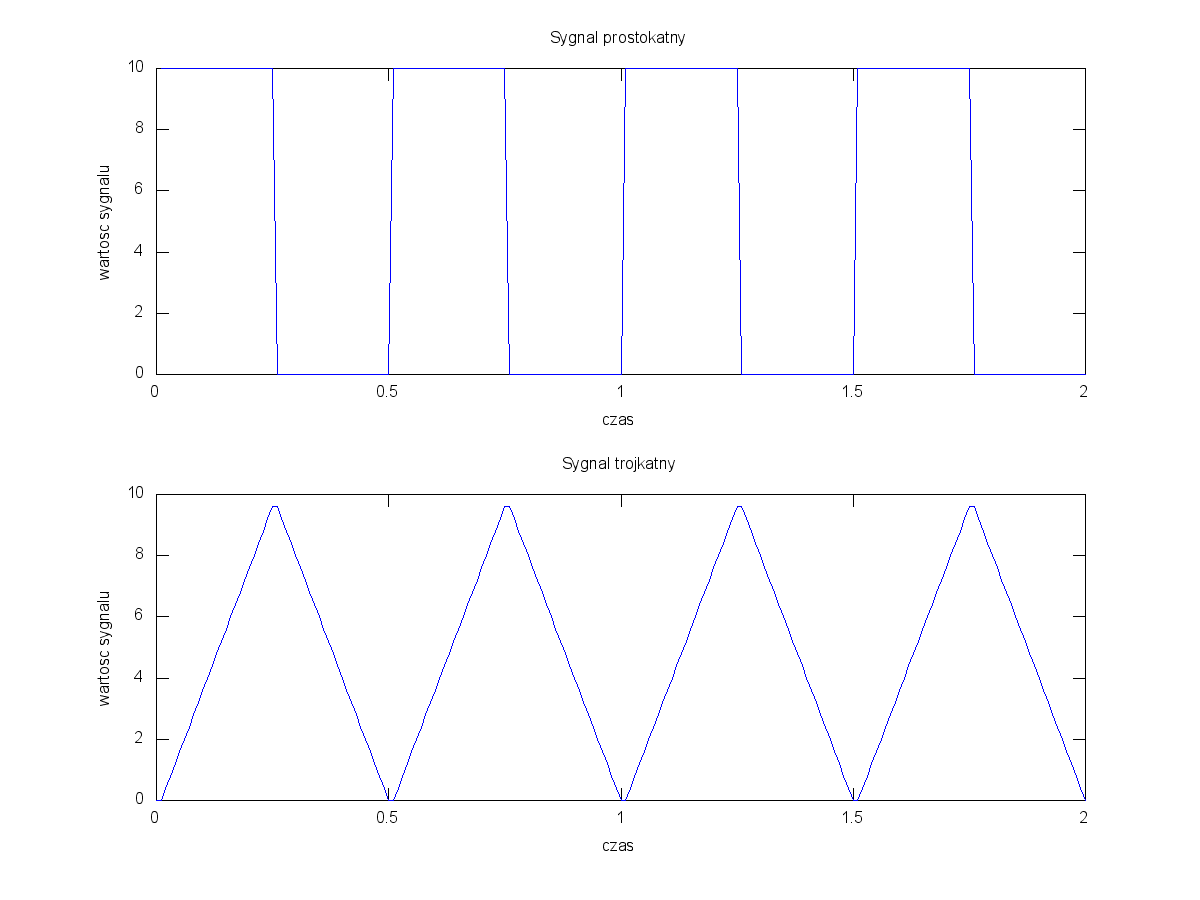
\includegraphics[scale=.5]{out/Figure1.png}
  %       \caption{\label{wykres1}Badane sygnały.}
  %     \end{center}
  %   \end{figure}
  % \end{landscape}
  
% Wykresy (end)
\end{document}
